\documentclass[12pt, a4paper]{extarticle}


% Russian text support
\usepackage[T2A]{fontenc}
\usepackage[utf8]{inputenc}
\usepackage[russian]{babel}

% Some useful packages
\usepackage{indentfirst}
\usepackage{etoolbox}
\usepackage{amsmath}
\usepackage{amssymb}
\usepackage{amsfonts}
\usepackage{xcolor}
\usepackage{indentfirst}
\usepackage{listings}
\usepackage{mathtools}

% Codestyle
\definecolor{codegreen}{rgb}{0,0.6,0}
\definecolor{codegray}{rgb}{0.5,0.5,0.5}
\definecolor{codepurple}{rgb}{0.58,0,0.82}
\definecolor{backcolour}{rgb}{1,1,1}

\lstdefinestyle{mystyle}{
    backgroundcolor=\color{backcolour},   
    commentstyle=\color{codegreen},
    keywordstyle=\color{magenta},
    numberstyle=\tiny\color{codegray},
    stringstyle=\color{codepurple},
    basicstyle=\ttfamily\footnotesize,
    breakatwhitespace=false,         
    breaklines=true,                 
    captionpos=b,                    
    keepspaces=true,                 
    numbers=left,                    
    numbersep=5pt,                  
    showspaces=false,                
    showstringspaces=false,
    showtabs=false,                  
    tabsize=2
}

\lstset{style=mystyle}

% Pictures support
\usepackage{graphicx}
\graphicspath{ {./pictures/} }

% Page geometry
\usepackage[
    left=3cm,
    right=1cm,
    top=2cm,
    bottom=2cm
]{geometry}

% Make titles not to have numbering
\newenvironment*{dummyenv}{}{}

\newcommand{\mysection}[1]{
    \addcontentsline{toc}{section}{#1}
    \begin{dummyenv}
        \bfseries\large #1
    \end{dummyenv}
}

\makeatletter
\patchcmd{\l@section}
  {\hfil}
  {\leaders\hbox{\normalfont$\m@th\mkern \@dotsep mu\hbox{.}\mkern \@dotsep mu$}\hfill}
  {}{}
\makeatother

% Useful commands
\newcommand{\Sum}[2]{\sum\limits_{#1}^{#2}}

% Here we go...
\title{БДЗ по анализу данных и машинному обучению}
\author{Фирсов Георгий, М21-507}

\begin{document}

\maketitle

\begin{center}
    \textbf{Вариант}: 10
\end{center}

\tableofcontents

\pagebreak

\mysection{Задание 1}

Построить двухслойную нейронную сеть, реализующую булеву функцию 
$f(x_1, x_2, x_3) = (x_1 \land x_2) \oplus (x_2 \land \overline{x_3}) \lor (x_1 \lor \overline{x_3})$.

Для данной функции несложно получить минДНФ: $f(x_1, x_2, x_3) = x_1 \lor \overline{x_3}$. 
Явственно видно, что существенно $f$ зависит только от $x_1$ и $x_3$, а значит в сети все
синаптические коэффициенты при $x_2$ положим равными нулю.

Перепишем в обозначениях Айверсона и через арифметические операции: $f(x_1, x_2, x_3) = 
\left[x_1 - x_3 + \frac{1}{2} > 0\right]$, что в целом реализуется и одним слоем,
но требуется двухслойная сеть, поэтому первый слой вычисляет $\overline{x_3}$, а второй -- реализует
дизъюнкцию. Таким образом \textit{двухслойная} нейронная сеть, вычисляющая функцию $f$, будет 
выглядеть согласно рисунку \ref{fig:task-1} (связи с нулевыми синаптическими коэффициентами не показаны).

\begin{figure}[h!]
    \centering
    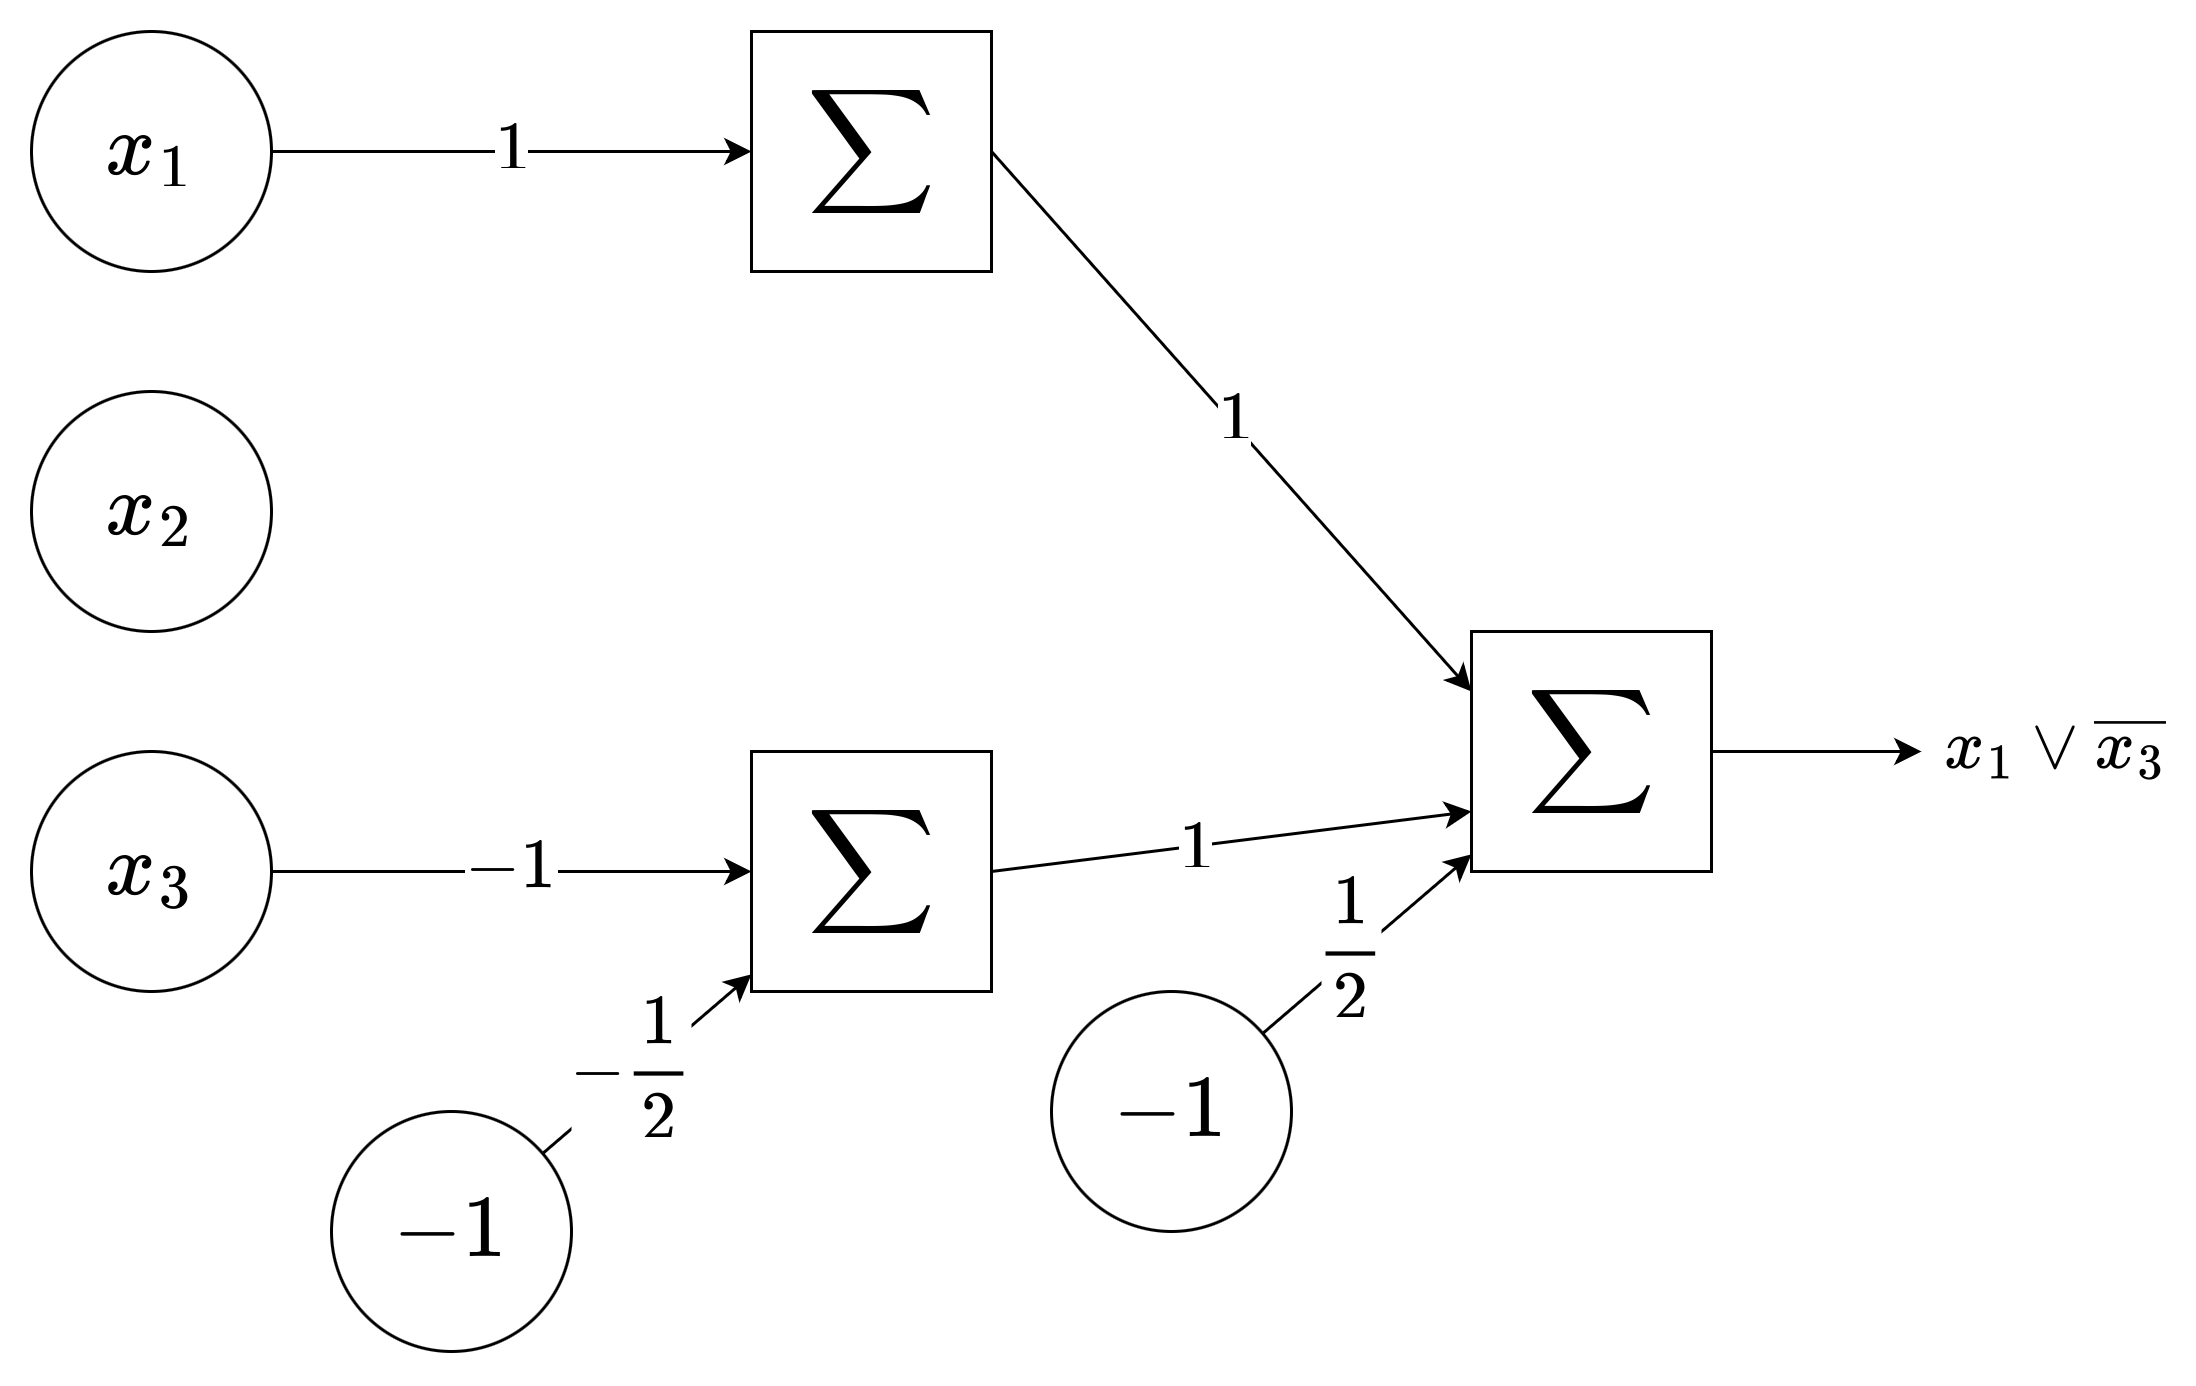
\includegraphics[width=0.8\textwidth]{task-1.png}
    \caption{Нейронная сеть, вычисляющая функцию $x_1 \lor \overline{x_3}$.}
    \label{fig:task-1}
\end{figure}

\mysection{Задание 2}

Исходные данные:
\begin{table}[h!]
    \centering
    \begin{tabular}{|c|c|c|c|c|c|c|c|c|c|c|}
        \hline
        $t$ & 1 & 2 & 3 & 4 & 5 & 6 & 7 & 8 & 9 & 10 \\
        \hline
        $X_t$ & 12 & 36 & 25 & 18 & 41 & 34 & 56 & 49 & 50 & 62 \\
        \hline
    \end{tabular}
\end{table}

Требуется в сущности найти коэффициент корреляции Пирсона между $X$ и $L^3 X$, где $L$ --- оператор лага.
Рассчитаем данный коэффициент (а точнее его оценку по выборке):
\begin{equation}
\begin{split}
    \hat{r}_{X, L^3 X} 
    & = \frac{\mathbb{E}[X\cdot L^3 X] - \mathbb{E}[X]\mathbb{E}[L^3 X]}{s_{X} s_{L^3X}} = 
        \frac{\frac{1}{n - 3}\Sum{j = 4}{n}x_j x_{j - 3} - 
        \frac{1}{(n - 3) ^ 2}\left(\Sum{j = 4}{n}x_j\right)\left(\Sum{j = 4}{n}x_{j - 3}\right)}
        {\sqrt{\frac{1}{n - 3}\Sum{j = 4}{n}\left(x_j - \mathbb{E}[L^3 X]\right) ^ 2} 
        \sqrt{\frac{1}{n - 3}\Sum{j = 4}{n}\left(x_{j - 3} - \mathbb{E}[X]\right) ^ 2}}.
\end{split}
\label{eq:autocorr}
\end{equation}

Вычислим необходимые величины:
\begin{equation*}
\begin{split}
    \mathbb{E}[X] & = \frac{12 + 36 + 25 + 18 + 41 + 34 + 56}{7} = 31.714285714285715 \\
    \mathbb{E}[L^3 X] & = \frac{18 + 41 + 34 + 56 + 49 + 50 + 62}{7} = 44.285714285714285 \\
    \mathbb{E}[X\cdot L^3 X] & = \frac{216 + 1476 +  850 + 1008 + 2009 + 1700 + 3472}{7} = 1533 \\
    s_{X} & = \sqrt{\frac{388.65306122 + 18.36734694 + \cdots + 
        589.79591837}{7}} \approx 13.739560044050961 \\
    s_{L^2X} &= \sqrt{\frac{690.93877551 + 10.79591837 + \cdots + 
        313.79591837}{7}} \approx 13.697906886134994
\end{split}
\end{equation*}

Тогда согласно (\ref{eq:autocorr}):
\begin{equation}
    \hat{r}_{X, L^3 X} = \frac{1533 - 31.714285714285715 \cdot 44.285714285714285}{
        13.739560044050961 \cdot 13.697906886134994} = 0.6828268298655353.
\end{equation}

\textbf{Ответ}: $\hat{r}_{X, L^3 X} = 0.6828268298655353$.
\\

\mysection{Задание 3}

Исходные данные:
\begin{table}[h!]
    \centering
    \begin{tabular}{|c|c|c|c|c|c|c|c|c|c|c|}
        \hline
        $t$ & 1 & 2 & 3 & 4 & 5 & 6 & 7 & 8 & 9 & 10 \\
        \hline
        $X_t$ & 235 & 217 & 197 & 221 & 175 & 168 & 192 & 154 & 132 & 178 \\
        \hline
    \end{tabular}
\end{table}

Для начала построим график временного ряда, чтобы определить тип тренда (рис. \ref{fig:task-3-ts}).

\begin{figure}[h!]
    \centering
    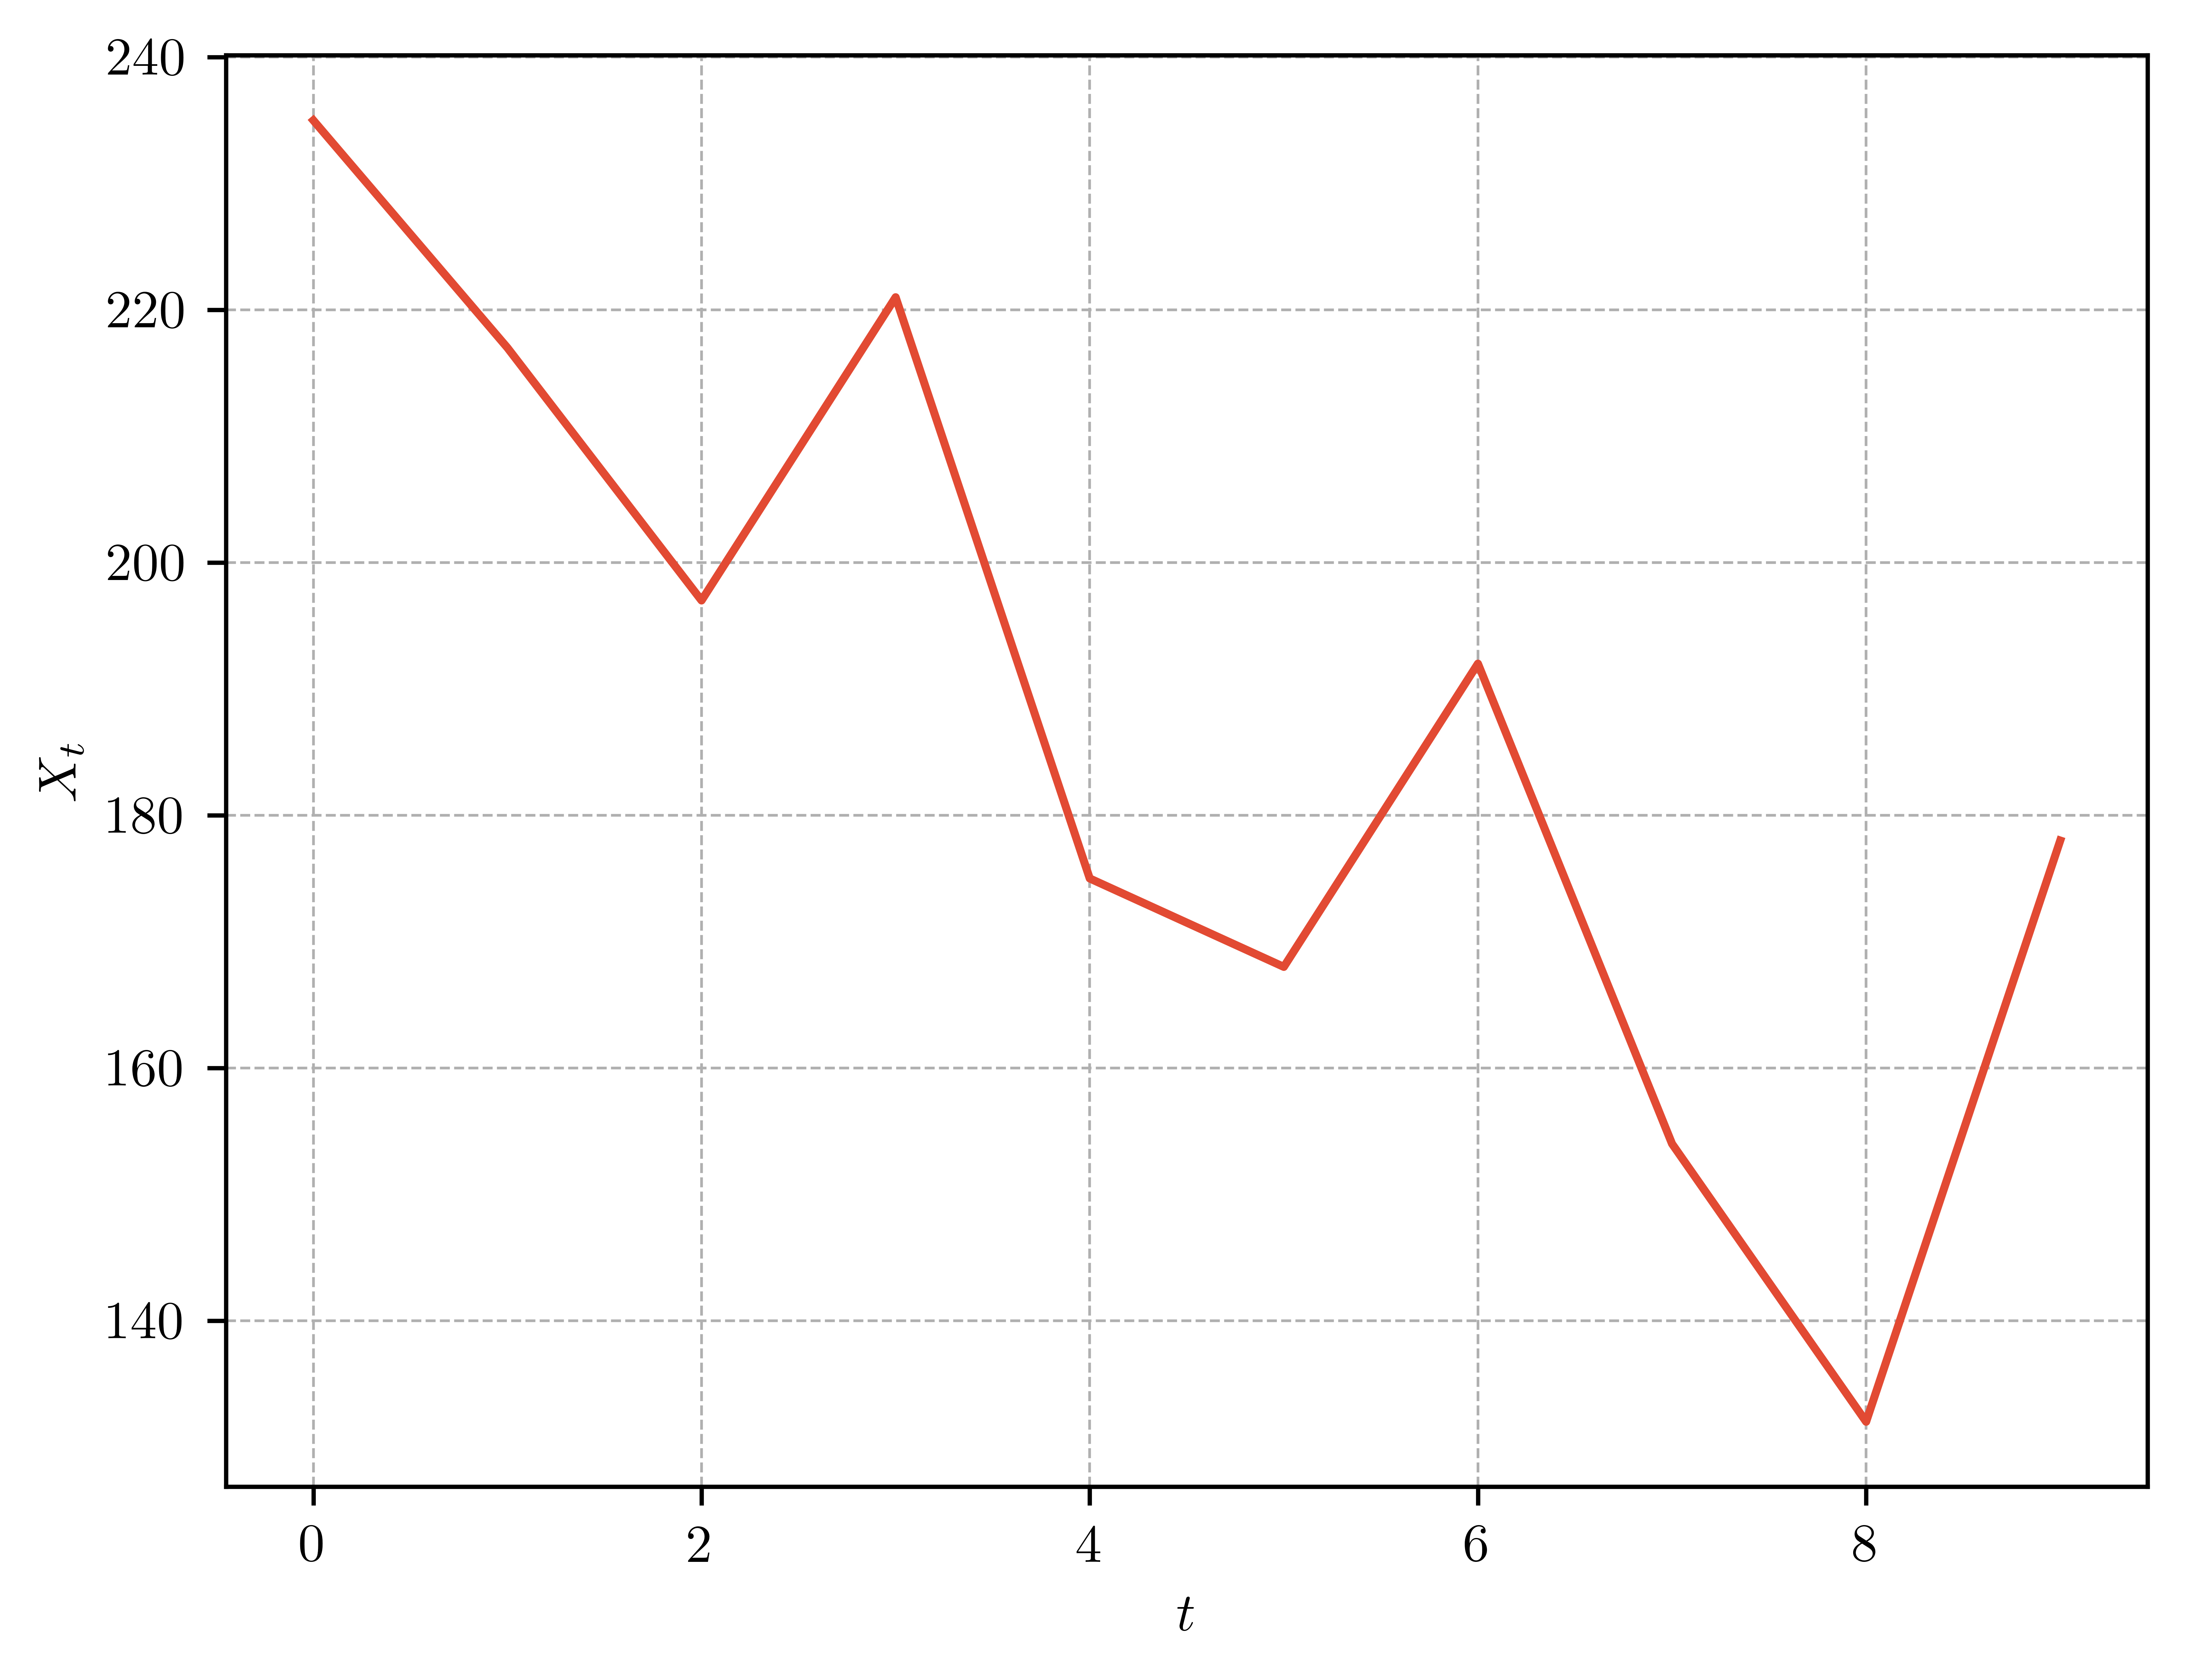
\includegraphics[width=0.7\textwidth]{task-3.png}
    \caption{График временного ряда}
    \label{fig:task-3-ts}
\end{figure}

Несложно видеть, что гетероскедастичность отсутствует, а значит тренд аддитивный и его можно найти,
самое простое, при помощи линейной регрессии $t$ на $X_t$ по формуле:
\begin{equation*}
    \text{F}^\top\text{F} \hat{\beta} = \text{F} y,
\end{equation*}
где $\text{F}$ --- регрессионная матрица (матрица плана), $y$ --- вектор значений временного ряда 
($y = (X_1,...,X_n) ^ \top$), $\hat{\beta}$ --- МНК-оценки коэффициентов регрессии.

В нашем случае регрессионная матрица будет иметь вид (с учетом того, что требуется также учесть
свободный член линейного уравнения):
\begin{equation*}
    \text{F} = \begin{Vmatrix}
        1 & 1 & 1 & 1 & 1 & 1 & 1 & 1 & 1 & 1  \\
        1 & 2 & 3 & 4 & 5 & 6 & 7 & 8 & 9 & 10
    \end{Vmatrix} ^ \top.
\end{equation*}

Тогда после несложных  вычислений получаем: $\hat{\beta} = (234.13333333, -8.58787879) ^ \top$. 
Построим оцененный тренд на фоне временного ряда (рис. \ref{fig:task-3-trend}).

\begin{figure}[h!]
    \centering
    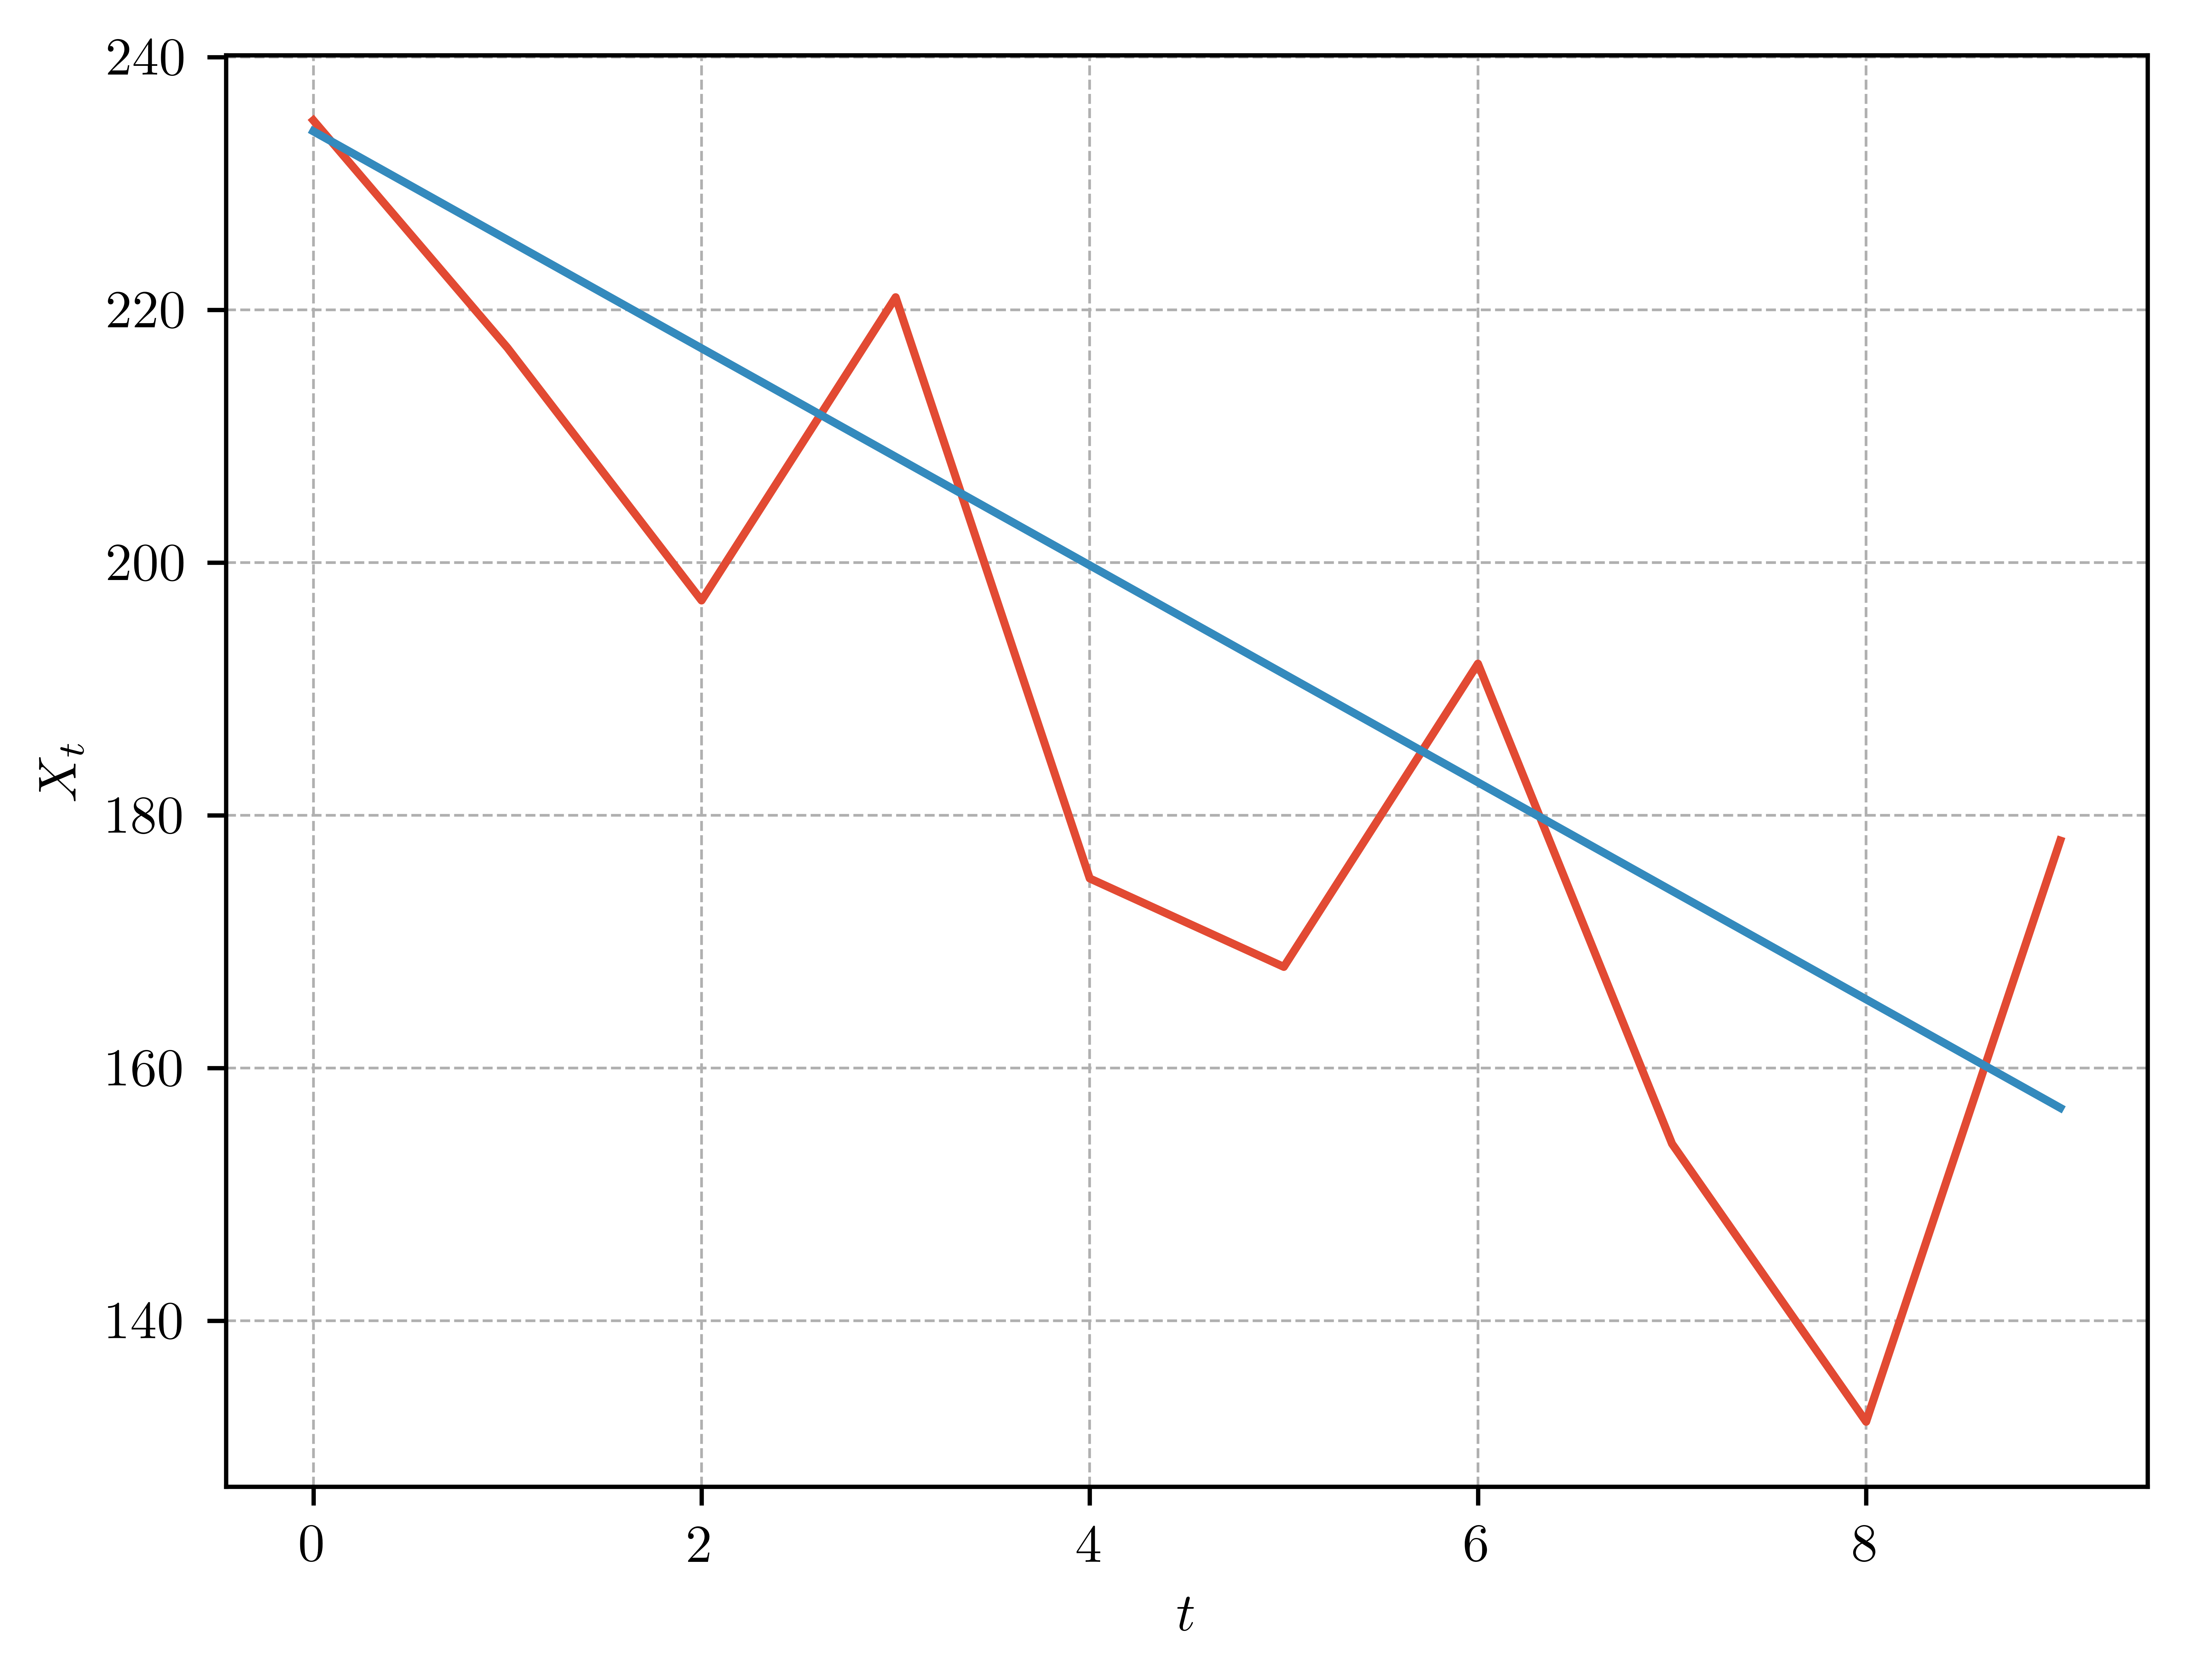
\includegraphics[width=0.7\textwidth]{task-3-trend.png}
    \caption{График временного ряда и его тренд}
    \label{fig:task-3-trend}
\end{figure}

\textbf{Ответ}: уравнение тренда: $234.13333333 - 8.58787879t$.
\\

\mysection{Задание 4}

Проведем некоторую предобработку данных, представиви $y$ в следующем виде:
\begin{equation*}
    y = \begin{Vmatrix}
        1 & 0 \\
        0 & 1 \\
        0 & 1 \\
        1 & 0
    \end{Vmatrix}.
\end{equation*}

Тогда после обучения матрицы весов и векторы сдвигов имеют вид:
\begin{equation*}
\begin{split}
    W_1 & = \begin{Vmatrix*}[r]
        -0.3513391 &  0.2577573 & -0.6137178 &  0.5554326 & -0.7433472 & 0.1489284 \\
         0.9980044 & -0.8825159 &  0.9700653 & -1.2001997 &  1.2608868 & 0.3367311 \\
        -0.2866572 &  0.1848346 & -0.1722901 &  0.3386492 & -0.2378174 & 0.1953463 \\
        -0.8526601 &  0.8139937 & -0.7290487 &  0.9301556 & -1.0092406 & 0.0954579
    \end{Vmatrix*} \\ 
    W_2 & = \begin{Vmatrix*}[r]
        -1.2977191 &  1.3870878 \\
         1.4359849 & -1.0272061 \\
        -1.3394972 &  1.3238781 \\
         1.8256082 & -2.1745731 \\
        -2.1831277 &  2.1162481 \\
         0.4879742 & -0.3353436
    \end{Vmatrix*}
\end{split}
\end{equation*}

\begin{equation*}
\begin{split}
    b_1 & = \begin{Vmatrix}
        -0.028159 & 0.14365459 & -0.12131796 & 0.12334835 & 0.17156292 & 0.15090948
    \end{Vmatrix} \\
    b_2 & = \begin{Vmatrix}
        0.24416564 & -0.43038426
    \end{Vmatrix}
\end{split}
\end{equation*}
\\

\mysection{Задание 5}

:(

\newpage
\mysection{Приложение А. Исходный код нейронной сети для задачи 4}

Исходный код написан на языке Python 3.11 с использованием библиотек numpy и scipy.
\begin{lstlisting}[language=python]
class TinyNeuralNetwork(object):
    def __init__(self):
        input_dim = 4
        intermediate_dim = 6
        output_dim = 2
        
        self.b1 = TinyNeuralNetwork._initialize_wights(intermediate_dim)
        self.W1 = TinyNeuralNetwork._initialize_wights(
            (input_dim, intermediate_dim))
            
        self.b2 = TinyNeuralNetwork._initialize_wights(output_dim)
        self.W2 = TinyNeuralNetwork._initialize_wights(
            (intermediate_dim, output_dim))
    
    
    def fit(self, X, y, *, lr=0.01, epoch=50):
        for _ in range(epoch):
            self._backprop(X, y, lr)
            
    
    def predict(self, X):
        output, _ = self._predict(X)
        return output
    
    
    def _predict(self, X):
        layer1 = TinyNeuralNetwork._sigmoid(np.dot(X, self.W1) + self.b1)
        output = TinyNeuralNetwork._sigmoid(np.dot(layer1, self.W2) 
            + self.b2)
            
        return output, layer1
    
    
    def _backprop(self, X, y, lr):
        output, layer1 = self._predict(X)
        
        prev_2 = 2 * (y - output) * TinyNeuralNetwork._sigmoid_prime(
            np.dot(layer1, self.W2) + self.b2)
        
        dW2 = np.dot(layer1.T, prev_2)
        db2 = prev_2.sum(axis=0)
        
        prev_1 = np.dot(prev_2, self.W2.T) * TinyNeuralNetwork._sigmoid_prime(np.dot(X, self.W1) + self.b1)
        
        dW1 = np.dot(X.T, prev_1)
        db1 = prev_1.sum(axis=0)
        
        self.W1 += lr * dW1
        self.W2 += lr * dW2

        self.b1 += lr * db1
        self.b2 += lr * db2
    
    
    @staticmethod
    def _initialize_wights(shape):
        return scipy.stats.uniform.rvs(loc=-0.25, scale=0.5, size=shape)
    
    
    @staticmethod
    def _sigmoid(X):
        return 1 / (1 + np.exp(-X))
    
    
    @staticmethod
    def _sigmoid_prime(X):
        s = TinyNeuralNetwork._sigmoid(X)
        return s * (1 - s)
\end{lstlisting}

\end{document}
